\documentclass[%
	fontsize=11pt,% bigger font
	paper=a4,% paper size
	pagesize,% set pagesize in PDF
	twoside=false,% =oneside
	listof=totoc,%add list of figures to toc
	draft% TODO remove this!
]{scrbook}

%---------------------------------------
%---------PACKAGES----------------------
%---------------------------------------

% language
\usepackage[english]{babel}

% font config
\usepackage{libertine}
\usepackage[T1]{fontenc}

% microtype
\usepackage[
	activate={true,nocompatibility},% activate protrusion and expansion
	final,% enable microtype; use "draft" to disable
	tracking=true,% activate these techniques
	kerning=true,% -''-
	spacing=nonfrench,% activate and supress warning
	factor=1100,% add 10% to the protrusion amount (default is 1000)
	stretch=10,% reduce stretchability/shrinkability (default is 20/20)
	shrink=10% -''-
]{microtype}

% links
\usepackage{hyperref}

% math
\usepackage{amsmath}
\usepackage{amssymb}

% graphics
\usepackage{tikz}
\usepackage{tikz-3dplot}
\usepackage{pgfplots}

% glossar
% dep: hyperref
\usepackage[
	toc% add to toc
]{glossaries}

% bibtex
% dep: hyperref
\usepackage[
	backend=biber,% nice fast backend
	style=alphabetic% how the shortcuts should look like
]{biblatex}

% units
% dep: amssymb
\usepackage{siunitx}

% TODO remove this!
% debug packages
\usepackage{blindtext}


%---------------------------------------
%---------SETTINGS----------------------
%---------------------------------------

% general informaion
\title{Some funny words}
\author{Marco Neumann}

% color
\definecolor{colcontrast}{RGB}{40,100,40}
\definecolor{colcontrast2}{RGB}{40,40,100}

% links
\hypersetup{
	colorlinks,% colored text instead of borders
	linkcolor=black,% black inter document links
	urlcolor=black,% black urls
	citecolor=black,% black cite
	final% also work in draft mode, TODO remove this!
}

% tikz
\usetikzlibrary{arrows}
\tikzset{
	>=stealth',
	axis/.style={->, very thick, >=stealth'}
}
\newcommand*\circled[1]{\tikz[baseline={($(char.south) + (0,0.5pt)$)}]{
	\node[shape=circle,draw,inner sep=0.5pt,font=\tiny,thick] (char) {\textsf{#1}};}}

% bibtex
\addbibresource{citiation.bib}

% math macros
\newcommand{\set}[1]{\mathbb{#1}}

% calculation helper
\newcommand{\mycalc}[2]{
	\pgfkeys{/pgf/fpu, /pgf/fpu/output format=fixed}
	\pgfmathparse{#2}
	\edef#1{\pgfmathresult}
	\pgfkeys{/pgf/fpu=false}
}


%---------------------------------------
%---------GLOSSARY----------------------
%---------------------------------------

\newglossaryentry{random number generator}
{
	name={Random Number Generator},
	description={Generates random numbers}
}

\newacronym{rng}{RNG}{\glslink{random number generator}{Random Number Generator}}

\makeglossaries% build glossary
\glsunsetall% fix acronyms


\begin{document}

\frontmatter
\maketitle
\tableofcontents

\mainmatter
\chapter{How to beat the system}
The method described in this thesis has some weaknesses. I will construct a dateset, which is not processed very well and I will discuss, why this type of data is not very common.

\section{Constructing a special dataset}\label{sec:constr}
Consider the following a dataset, that is made of many random points $(x, y, z) \in \left[0, 1\right)^3$, that satisfy the following constraint:
\begin{equation}\label{eq:beat}
	(x + y + z) \bmod 1 = 0
\end{equation}
The points are uniform distributed if you project them on one or two dimensions. But if you calculate the three dimensional distribution, the points do not show a uniform distribution. (see Figure~\ref{fig:beat}). Because the generated points have two degrees of freedom, the two dimensional distribution test will fail. It is also possible to generate datasets with even more degrees of freedom using the same technique.\footnote{You may not be able to imagine datasets with more than three dimensions. For 4 dimensions, you find some help: \url{http://crepererum.github.io/brain4D/\#constructed.csv}}
\begin{figure}
	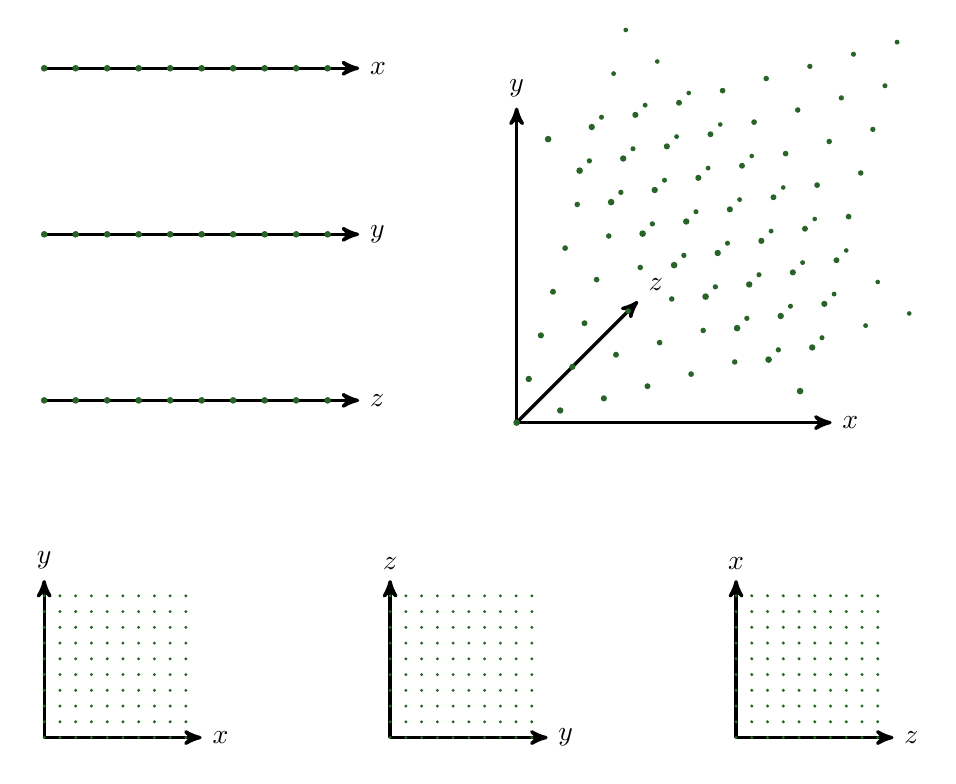
\begin{tikzpicture}[scale = 5.0]
	\begin{scope}
		\foreach \name [count=\d from 0] in {x,y,z} {
			\begin{scope}[yshift=-\d*12]
				\begin{scope}[scale=0.8]
					\draw[axis] (0,0) -- (1,0) node[right]{$\name$};
					\foreach \x in {0,...,9} {
						\fill[colcontrast] (\x/10,0) circle(0.3pt);
					}
				\end{scope}
			\end{scope}
		}
	\end{scope}
	\begin{scope}[shift={(0,-1.7)}]
		\foreach \namefirst/\namesecond [count=\d from 0] in {x/y,y/z,z/x} {
			\begin{scope}[xshift=\d*25]
				\begin{scope}[scale=0.4]
					\draw[axis] (0,0) -- (1,0) node[right]{$\namefirst$};
					\draw[axis] (0,0) -- (0,1) node[above]{$\namesecond$};
					\foreach \x in {0,...,9} {
						\foreach \y in {0,...,9} {
							\fill[colcontrast] (\x/10,\y/10) circle(0.3pt);
						}
					}
				\end{scope}
			\end{scope}
		}
	\end{scope}
	\begin{scope}[shift={(1.2,-0.9)}]
		\begin{scope}[scale=0.8]
			\draw[axis] (0,0,0) -- (1,0,0) node[right]{$x$};
			\draw[axis] (0,0,0) -- (0,1,0) node[above]{$y$};
			\draw[axis] (0,0,0) -- (0,0,-1) node[above right]{$z$};
			\foreach \x in {0,...,9} {
				\foreach \y in {0,...,9} {
					\pgfmathsetmacro{\z}{mod(\x+\y,10)}
					\fill[colcontrast] (\x/10,\y/10,-\z/10) circle(0.3pt-0.1pt*\z/10);
				}
			}
		\end{scope}
	\end{scope}
\end{tikzpicture}


	\caption{Situation described in Equation~\ref{eq:beat}}
	\label{fig:beat}
\end{figure}

The problem occures every time, when the dataset contains a subspace with $n \in \set{N}_+$ Dimensions but $m \in \left\{1,\dots,n-1\right\}$ degrees of freedom. Furthermore the dependency of each dimension on the degrees of freedom has to be equal.

\section{Handling this issue}
Because it datasets with generated dimensions are not very uncommon, I will propose a simple method to handle them. To get a good perfomance on high dimensional datasets, it is not possible to check distributions in subspaces where the size depends on the number of all dimensions. But as shown in \cite{journals/prl/SharmaP07}, a PCA can be computed in $O\left( d^2h + d^2n \right)$ where $h$ is the number of degrees of freedom. After this step, the algorithm will find the most common subspaces.


\chapter{Datasets}
High dimensional datasets are not a very common research topics. In this chapter I will describe some data sources and possible applications of the described algorithm. I also show some interpretations of subspaces in different datasets and some failed approaches of finding them. To get, isolate and preprocess the data I've used some scripts. Because I think open research should not only contain open publications but also open data sources, you can find the scripts and some notes about them online.\footnote{\url{https://github.com/crepererum/GSD}} Should you have some questions, find a bug or want to contribute, feel free to use the issue tracker or file a pull request.

\section{Audio Spectrum}
An audio spectrum can characterize the underlying material. I analyzed the songs from the following collections:
\begin{itemize}
	\item Daft Punk -- Random Access Memories (\circled{P}2013 by Daft Life, Columbia), \num{13} songs
	\item Mayday 2013 -- Never Stop Raving (\circled{C}2013 by Contor Records GmbH), \num{60} songs
\end{itemize}
I converted the audio to a sample rate of \SI{44100}{\hertz}. After it, I splitted the audio files into parts containing \num{4096} parts, applied the Hamming window and passed it to a FFT. The FFT produces a output vector with \num{4096} values, but only \num{2048} values are usable, because the spectrum should be mirrored. The values are normalized and converted to \si{\decibel}. Then I calculated the mean of \num{32} parts to supress noise, which is a common audio effect in modern music, but may also effect classical records. This mean vector has a length of \num{2048} and is written to a file. So, the mean of \num{32} parts is one data element. Figure~\ref{fig:audio} shows some of the results.
\begin{figure}
	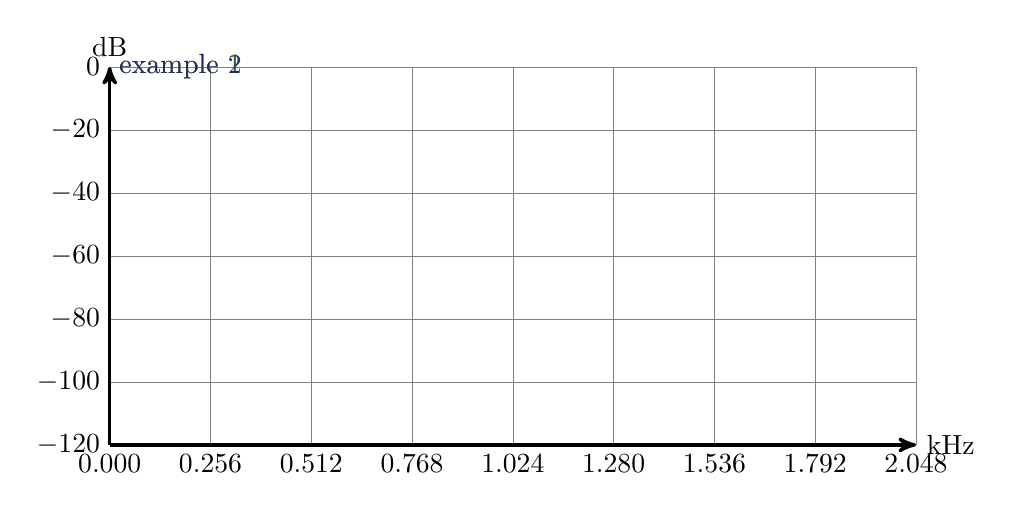
\begin{tikzpicture}
	\def\xmin{0}
	\def\xmax{2.048}
	\def\xstep{0.2}
	\def\ymin{-120}
	\def\ymax{0}
	\def\ystep{5}

	\begin{scope}[xscale=5,yscale=0.04]
		\draw[style=help lines, ystep=20, xstep=0.256] (\xmin,\ymin) grid(\xmax,\ymax);

		\foreach \x in {\xmin,0.256,...,\xmax} {
			\node at (\x,\ymin) [below]{\num[round-precision=3,round-mode=places]{\x}};
		}
		\foreach \y in {\ymin,-100,...,\ymax} {
			\node at (\xmin,\y) [left]{\num{\y}};
		}

		\draw[colcontrast] plot[smooth] file{data/audio1.dat} node[right]{example 1};
		\draw[colcontrast2] plot[smooth] file{data/audio2.dat} node[right]{example 2};

		\draw[axis] (\xmin,\ymin) -- (\xmax,\ymin) node[right]{\si{\kilo\hertz}};
		\draw[axis] (\xmin,\ymin) -- (\xmin,\ymax) node[above]{\si{\decibel}};
	\end{scope}
\end{tikzpicture}


	\caption{Audio spectrum}
	\label{fig:audio}
\end{figure}

The subspace analyzis performance well but gives boring results. Meanly the first and last bins of the spectrum forms one subsapce and the middle part describes another.

\section{Drug Database}


\appendix


\backmatter

\listoffigures

\printglossaries

\cleardoublepage
\phantomsection
\addcontentsline{toc}{chapter}{Bibliography}
\printbibliography

\end{document}

